\section{Approach}
\subsection{Simulated Network}

The network of our simulation is designed to give a real-time nature to the data transfer between the Tennesee Eastman(TE) physical simulation and the TE Controller. Both the controller and simulation are written in Matlab and connected to our network with the OMNeTBridge Class. (These are described in later sections.)

The network is based primarly on two factory level components, sensors and actuators, that send data to a remote facility that sends back control signals. This is based on most SCADA systems that need remote facilites to monitor their data. These signals are sent over a simulated "Internet" that allows accurate packet loss, bit errors and data rates. 

Due to limitations of the default Inet packets we are not actually sending the data through the network. Rather, the packets the controller recieves act as a trigger to have the controller update the data from that sensor, and send an update to the actuators if need be. 

The actual implementation of these components is discribed in later sections. 


\subsection{Controller}


\subsubsection{Actuator}

The actuator acts as a server which recieves an update packet from the controller, grabs its appropriate data fron the conroller OMNeTBridge and then passes it to the correct function.

\subsubsection{Sensor}


The Sensor is a relatively simple module that sends an update signal based on a timer. This is to model the refresh rate of most sensors. We have assumed that all sensors and network controllable and are able to tirelessly connect to a local access point via 802.11 Wireless LAN(WiFi). 

These modules send a TCP packet to a known IP address which in turn triggers the controller to update. This is a non-ideal method of updating as it does not allow correct implementation of attacking the data on the network. Ideally INET's TCP packets would allow us to send data to them, however as some modules are currently implemented deep copies are not done of messages or inappropriate casts are used. Future work should be planned to modify these modules or find a more correct
implementation of INET messages that allow custom data fields to be created and sent. 

\subsubsection{Internet Cloud}

\subsubsection{Factory Access Point}

\subsubsection{Factory Bridge}

\subsection{Matlab Simulation}

\subsubsection{Tennessee Eastman}

\subsection{C++ to Matlab Bridge}




\begin{figure*}
        \centering
		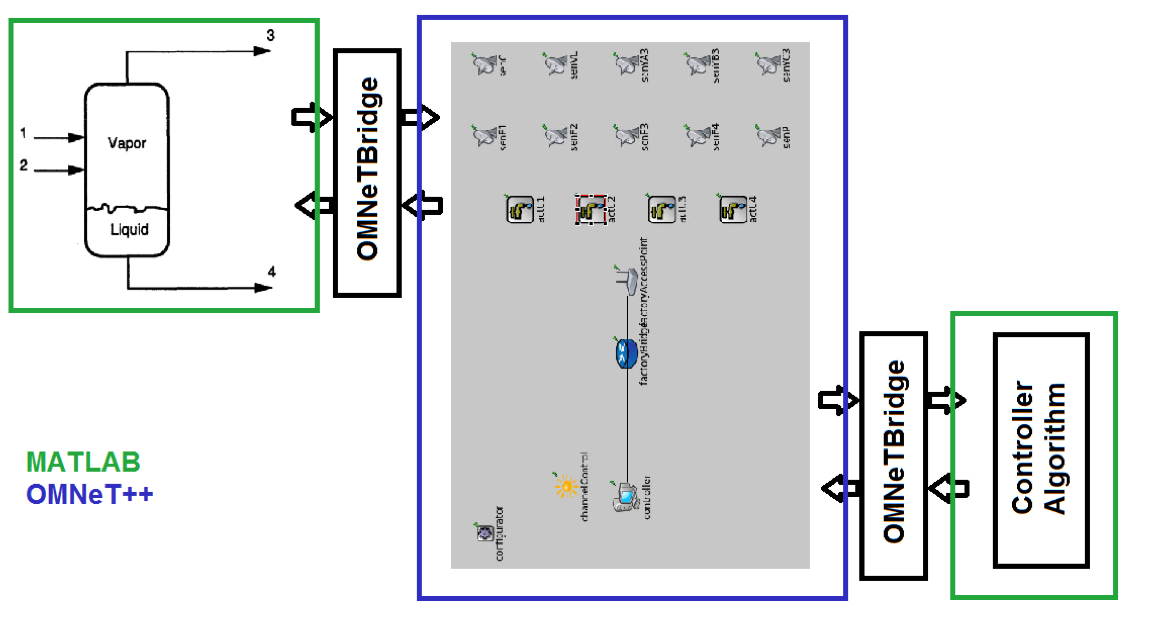
\includegraphics[width=0.8\textwidth]{figs/system.png}
        \caption{System Diagram.}
        \label{fig:system}        
\end{figure*}
